\documentclass{beamer}
\usepackage{graphicx}
\usetheme{Rochester}
\usepackage{minted}
\definecolor{bg}{rgb}{0.95,0.95,0.95}
\usepackage{graphics}
\usepackage{trfsigns}

\usepackage[absolute,overlay]{textpos}
\newenvironment{reference}[2]{%
  \begin{textblock*}{\textwidth}(#1,#2)
    \footnotesize\it\bgroup\color{blue!50!black}}{\egroup\end{textblock*}}

\setbeamertemplate{navigation symbols}{}

\title{CPFSK Softwareradio}
\author{Luckas Becker, Tobias Frahm}
\institute[HAW]{Dept. Informations- und Elektrotechnik\\HAW Hamburg}
\date{\today}

\begin{document}

\frame[plain]{\titlepage}

\section[Outline]{}

\frame{\tableofcontents}

\section{Softwareradio}

\frame{
  \frametitle{Softwareradio}
  \begin{itemize}
  \item<1-> Was ist der Unterschied zu einem normalen Empfänger?
  \end{itemize}
}

\section{Signalfluss Empfänger}
\frame{
  \frametitle{Signalfluss Empfänger}
  \begin{columns}
    \begin{column}{0.3\textwidth}
       \begin{itemize}
         \item 1. FIR-Polyphasen Bandpass
         \item 2. komplexes Kammfilter
         \item 3. FM-Verzögerungsdemodulator
         \item 4. Decodierer
       \end{itemize}
    \end{column}
    \begin{column}{0.8\textwidth}
        \begin{center}
         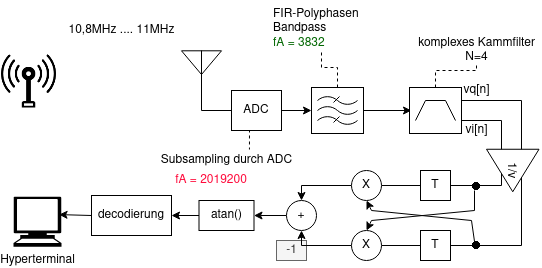
\includegraphics[width=0.6\textwidth]{images/signalfluss.png}
         \end{center}
    \end{column}
  \end{columns}
}

\section{FIR-Polyphasen Bandpass}
\frame{
	\frametitle{Softwareradio}
	\begin{itemize}
		\item<1-> Was ist der Unterschied zu einem normalen Empfänger?
	\end{itemize}
}
\section{Hilbert Transformator}
\section{Komplexes Kammfilter}
\section{FM-Verzögerungsdemodulator}
\section{Dekodierer}
\frame{
	\frametitle{Theorie Dekodierer}
	
	\begin{figure}
		\centering
		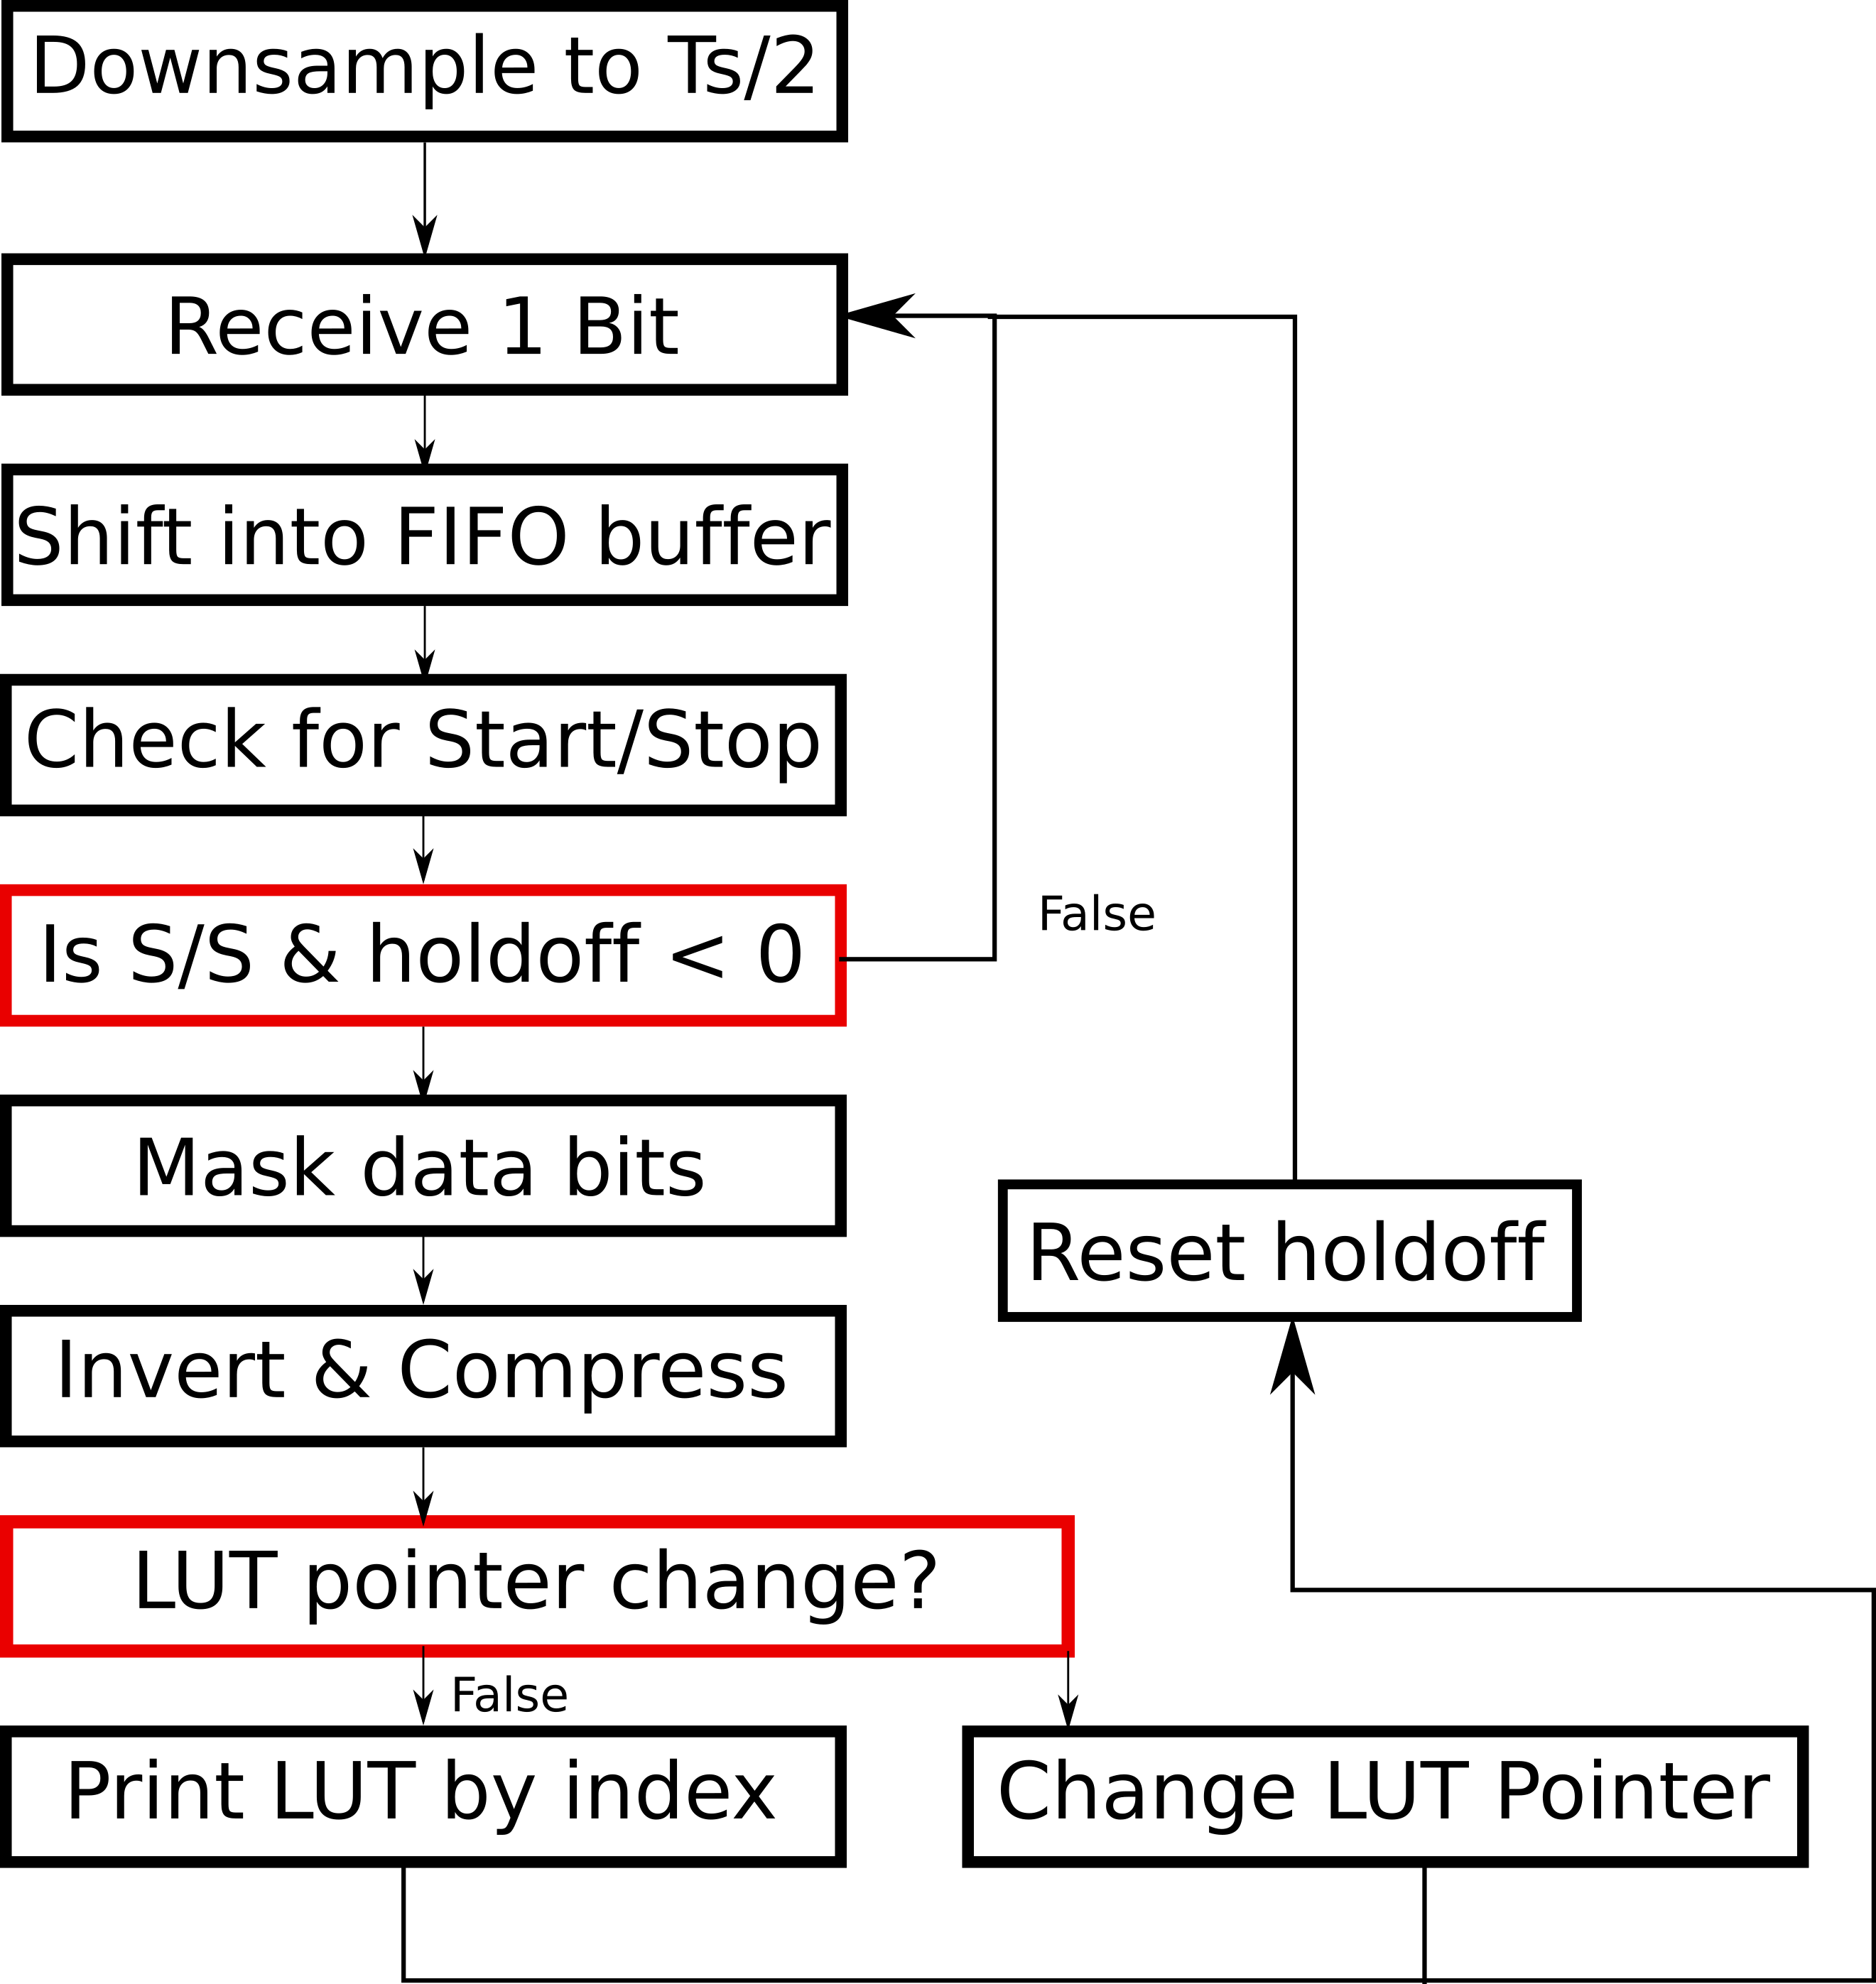
\includegraphics[width=0.7\linewidth]{images/rect833}
		\caption{}
		\label{fig:rect833}
	\end{figure}
	
}

\begin{frame}
	\frametitle{Implementierung Dekodierer}
	
%	\begin{listing}
%	\begin{minted}[linenos, bgcolor=bg, breaklines]{c}
%		void decode(unsigned short bit) {
%			
%			if (!current_lut) 
%			current_lut = lookup_char;
%			
%			buffer = buffer << 1;
%			buffer = buffer | bit;
%			startstop = buffer & 0x001F;
%			
%			if (startstop_holdoff > 0) // Underflow protection
%			startstop_holdoff -= 1;
%			
%			if (startstop == STOP_SEQUENCE && startstop_holdoff == 0) {
%				startstop_holdoff = 11;
%				// Shift over the start and stop section
%				// and mask the 10 message bits
%				index_pre = (buffer >> 5) & 0x03FF; 
%				// Compress bit stream to half its size
%				// Turn this 1 1 1 1 0 0 1 1 0 0 into 1 1 0 1 1
%				real_index = (((index_pre >> 0) & 0x0001) << 4) 
%				| (((index_pre >> 2) & 0x0001) << 3) 
%				| (((index_pre >> 4) & 0x0001) << 2) 
%				| (((index_pre >> 6) & 0x0001) << 1) 
%				| (((index_pre >> 8) & 0x0001) << 0);
				
%				if (real_index == SWITCH_TO_CHAR) {
%					// Change to characters
%					current_lut = lookup_char;
%				} else if (real_index == SWITCH_TO_NUM) {
%					// Change to numbers
%					current_lut = lookup_num;
%				} else {
%					#ifdef USE_MSVC_ANSI_C_SIM
%					// Everything else is a valid character
%					printf(" >> %c <<\n",current_lut[real_index-1]); 
%					#endif
%				}
%			}
%		}
%	\end{minted}
%\end{listing}

\end{frame}



\nocite{*} % Include everything in the .bib file.

\bibliographystyle{plainnat}
\bibliography{presentation}

% that's all, folks
\end{document}
